\documentclass{article}
\usepackage[subpreambles=true]{standalone}
\usepackage{graphicx}
\usepackage{amsmath,amssymb}
\usepackage{tikz}
\usetikzlibrary{decorations.pathreplacing,angles,quotes,shapes.geometric, arrows,calc}
\usepackage{caption}
\usepackage{subcaption}
\usepackage{wrapfig, blindtext}
\usepackage{pgfplots}
\usepackage{tikz}
\usetikzlibrary{decorations.pathreplacing,angles,quotes,shapes.geometric, arrows,calc}
\usepackage{import}
\pgfplotsset{compat=1.16}

\begin{document}
\begin{figure}[h!]
\begin{subfigure}[b]{0.30\linewidth}
   \begin{subfigure}[b]{1\linewidth}
   	\centering
	\resizebox{\linewidth}{!}{
 	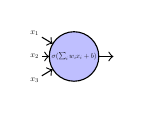
\begin{tikzpicture}		
		    \node[scale=0.3] 		   (x1) at (0,0.8) {$x_1$}; 
		    \node[scale=0.3] 		   (x2) at (0,0.5) {$x_2$};  
		    \node[scale=0.3] 		   (x3) at (0,0.2) {$x_3$};       
    		    \node [draw, circle,scale=0.18,fill=blue!25]          (c3) at (0.5,0.5) {\Large $\sigma(\sum_i w_i x_i + b)$};
    \draw[->] (x1)--(c3);
    \draw[->] (x2)--(c3);
    \draw[->] (x3)--(c3);
     \draw[->] (c3)--(1,0.5);
   	\end{tikzpicture}
	}
	\caption{}
	 \label{fig:perceptron}
 \end{subfigure}
 
   \begin{subfigure}[b]{1\textwidth}
  	\centering
	\resizebox{\linewidth}{!}{
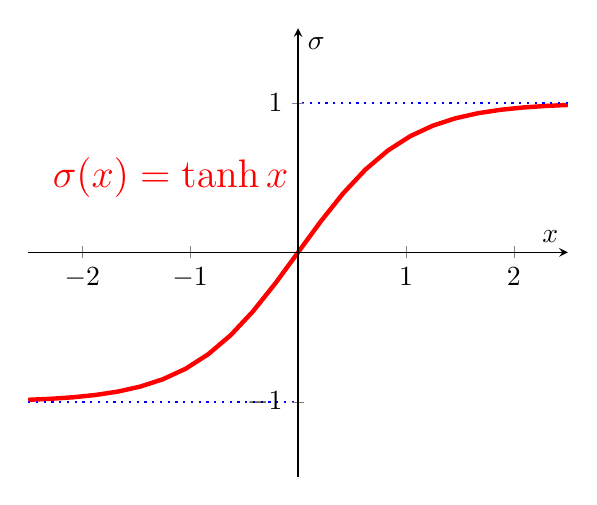
\begin{tikzpicture}
\begin{axis}[
    xmin=-2.5, xmax=2.5,
    ymin=-1.5, ymax=1.5,
    axis lines=center,
    axis on top=true,
    domain=-2.5:2.5,
    ylabel=$\sigma$,
    xlabel=$x$,
    ]

    \addplot [mark=none,draw=red,ultra thick] {tanh(\x)};
    \node [left, red] at (axis cs: 0,0.5) {\Large $\sigma(x) = \tanh x$};

    %% Add the asymptotes
    \draw [blue, dotted, thick] (axis cs:-2.5,-1)-- (axis cs:0,-1);
    \draw [blue, dotted, thick] (axis cs:+2.5,+1)-- (axis cs:0,+1);
\end{axis}
\end{tikzpicture}
	}
	\caption{}
	 \label{fig:tanh}
\end{subfigure}
\end{subfigure}
	 \begin{subfigure}[b]{0.70\textwidth}
\centering
\resizebox{\linewidth}{!}{
\def\layersep{1.5cm}
\begin{tikzpicture}[shorten >=1pt,draw=black, ->,node distance=\layersep]


    \tikzstyle{every pin edge}=[<-,shorten <=1pt]
    \tikzstyle{neuron}=[circle,draw=black, very thick, fill=blue!25, minimum size=22pt,inner sep=0pt]
    \tikzstyle{input neuron}=[circle,draw=black,very thick,fill=black!25, minimum size=22pt,inner sep=0pt];
    \tikzstyle{output neuron}=[neuron];
    \tikzstyle{hidden neuron}=[circle,draw=black,very thick,fill=blue!25,minimum size=22pt,inner sep=0pt];
    \tikzstyle{annot} = [text width=4em, text centered]

    % Draw the input layer nodes
    \foreach \name / \y in {1,...,5}
    % This is the same as writing \foreach \name / \y in {1/1,2/2,3/3,4/4}
        \node[input neuron] (I-\name) at (0,-\y) {$x_{\name}$};

    % Draw the hidden layer nodes
    \foreach \name / \y in {1,...,3}
        \path[yshift=-1cm]
            node[hidden neuron] (H-\name) at (\layersep,-\y cm) {};
            
  \foreach \namee / \y in {1,...,3}
        \path[yshift=-1 cm]
            node[hidden neuron] (H1-\namee) at (2*\layersep,-\y cm){};

           
    % Draw the output layer node
  \node[output neuron,pin={[pin edge={->}]right:}, right of=H1-2] (O) {};
    % Connect every node in the input layer with every node in the
    % hidden layer.
    \foreach \source in {1,...,5}
        \foreach \dest in {1,...,3}
            \path (I-\source) edge (H-\dest);

 \foreach \source in {1,...,3}
        \foreach \dest in {1,...,3}
            \path (H-\source) edge (H1-\dest);
            
    % Connect every node in the hidden layer with the output layer
    \foreach \source in {1,...,3}
        \path (H1-\source) edge (O);

    % Annotate the layers
    %\node[annot,above of=H-1, node distance=1cm] (hl) {Hidden layers};
   % \node[annot,left of=I-4] at (0) {Input layer};
    %\node[annot,right of=hl] {Output layer};
    
    \draw[decoration={brace,mirror,raise=15pt},decorate,-]
  (I-1.north) -- node[left=0.8cm,scale=0.7] {Input layer} (I-5.south);
 
    \draw[decoration={brace,raise=15pt},decorate,-]
  (H-1.west) --  node[above=0.8cm,scale=0.7]{Hidden layers}  (H1-1.east);
  
    \draw[decoration={brace,raise=15pt},decorate,-]
  (O.west) --  node[above=0.8cm,scale=0.7]{Output layers}  (O.east);
 
\end{tikzpicture}
}
 \caption{}
 \label{fig:network}
 \end{subfigure}

\caption{Neural Networks (a) A single neuron taking a vector of inputs and
returning a single output based on the weights, bias and activation function
of the network. (b) The hyperbolic tangent used as an activation
function.~\chris{is this the actual activation that you use in the GAN?
otherwise why focus on it alone, you could plot a handful on the same plot} (c)
A fully connected~\chris{you haven't mentioned what a fully connected network
actually is in the text} neural network containing two hidden layers that performs a
mapping of an input vector to a single output. \michael{Equation in the
neuron looks very small}~\chris{I agree, but the equation in (b) is even
smaller. I would also recommed that you make the style of the FC network hidden
and output layer neurons the same as the single perceptron in terms of colours.
You could put $x_i$s in the input layer.}}
\end{figure}

\end{document}

